\documentclass[a4paper]{IEEEtran}
\usepackage[slovene]{babel}
\usepackage[utf8]{inputenc}
\usepackage[T1]{fontenc}
\usepackage{amsfonts, amsthm,amsmath}
\usepackage{graphicx}
\usepackage{caption}
\usepackage{subcaption}
\title{Ravninske krivulje s pitagorejskim hodogramom}
\author{Jan Fekonja, Anže Marinko \\ IŠRM2, FMF \\ Predmet: Geometrijsko podprto računalniško oblikovanje}
\date{december 2018}
\newtheorem{theorem}{Izrek}
\newtheorem{remark}{Opomba}

\begin{document}
	\maketitle
	%\tableofcontents
	
	\section{Uvod}
	Hodogram parametrične krivulje $r (t)$ v $\mathbb{R}^n$ je odvod krivulje same $r\prime (t)$ podan kot parametrična krivulja. Polinomska krivulja $r (t)$ v $\mathbb{R}^n$ je krivulja s Pitagorejskim hodogramom (PH), če vsota kvadratov vseh $n$ polinomov na koordinatnih komponentah hodograma krivulje sovpada s kvadratom nekega polinoma $\sigma(t)$.
	Oglejmo si ravninske krivulje s PH.
	
	\section{Ravninske krivulje s Pitagorejskim hodogramom}
	Ključna lastnost, ki razlikuje ravninsko krivuljo s PH $r (t) = (x (t), y (t))$ od "navadne" polinomske krivulje je privzeta vključitev Pitagorejskega pogoja v svoj hodogram, in sicer komponente $r\prime (t) = (x\prime (t), y\prime (t))$ morajo zadoščati pogoju $$x\prime^2(t) + y\prime^2(t)= \sigma^2 (t)$$ za nek polinom $\sigma(t)$. To lastnost je dosežena z upoštevanjem sledeče karakterizacije Pitagorejskih trojic polinomov.
	\begin{theorem}
		Pitagorejski pogoj
		\begin{equation} \label{eq:1}
		a^2 (t) + b^2 (t) = c^2 (t)
		\end{equation}
		izpolnjujejo polinomi $a (t), b (t), c (t)$ natanko tedaj, ko jih lahko izrazimo z drugimi polinomi $u (t), v (t), w (t)$ v obliki
		\begin{eqnarray} \label{eq:2}
		a (t) &=& \lbrack u^2(t)-v^2(t)\rbrack w(t),\nonumber\\
		b(t) &=& 2u(t)v(t)w(t),\\
		c(t) &=& \lbrack u^2(t)+v^2(t)\rbrack w(t),\nonumber
		\end{eqnarray}
		kjer imata $u(t)$ in $v(t)$ paroma različne ničle.
	\end{theorem}
	\proof
	Očitno je pogoj \eqref{eq:2} zadosten za \eqref{eq:1}. Potrebnost pogoja pa je dokazana v \cite{knjiga} na strani 382.
	\endproof
	\begin{remark} 
		Rešitve, kjer je $w(t)$ konstantna, imenujejo primitivne Pitagorejske trojice.
	\end{remark}
	Tedaj je ravninska krivulja s PH $r (t) = (x (t), y (t))$ definirana z zamenjavo treh polinomov $u (t), v (t), w (t)$ v izrazih
	\begin{eqnarray}\label{eq:3}
	x\prime(t) &=& \lbrack u^2(t)-v^2(t)\rbrack w(t)\\
	y\prime(t)&=&2u(t)v(t)w(t)\nonumber
	\end{eqnarray}
	in z integriranjem.
	
	Vsak nekonstantni skupni faktor $u (t)$ in $v (t)$ lahko absorbiramo v $w (t)$. Poleg tega moramo dopustiti določene izbire za $w (t), u (t), v (t)$, ki dajejo "degenerirane" krivulje s PH:
	\begin{enumerate}
		\item če je $w (t) = 0$ ali $u (t) = v (t) = 0$, je dobljeni hodogram $x\prime (t) = y\prime (t) = 0$ in definira eno točko namesto zveznega loka,
		\item če so $w (t), u (t), v (t)$ vse konstante (z $w$ in vsaj eno od $u$, $v$ neničelno) dobimo enakomerno parametrizirano premico, trivialno krivuljo s PH,
		\item če sta $u (t)$ in $v (t)$ konstanti, kjer je vsaj ena različna od nič in $w (t)$ ni konstanta, je dobljen lok spet linearen, vendar njegova parametrična hitrost ni konstantna (v splošnem),
		\item prav tako nastanejo nekonstantno parametrizirani linearni loki (vzporedni z osjo x), če je $w (t)\not = 0$ in je eden od $u (t)$ in $v (t)$ nič.
	\end{enumerate}
	V nadaljevanju bomo obravnavali le primere, kjer so $w (t), u (t), v (t)$ vse neničelne,
	in $u (t), v (t)$ nista obe konstanti.
	\begin{remark}
		Če je $w$ polinom stopnje $\lambda$ in je $\mu$ večja izmed stopenj polinomov $u$ in $v$, je krivulja s PH dobljena z integracijo hodograma (\ref{eq:3}) stopnje $n = \lambda + 2\mu+ 1$.
	\end{remark}

	\section{B\'ezierjeve kontrolne točke krivulj s PH}
	Osredotočimo se predvsem na primitivne Pitagorejske hodograme ($u$ in $v$ brez skupne ničle, $w(t)=1$). Taki hodogrami definirajo regularne krivulje s PH, ki zadoščajo $r\prime (t)\not = 0$ za vse $t$. Točka na parametrični krivulji, kjer je $r\prime (t)=0$, je neregularna točka - običajno je to konica ali nenaden obrat tangente. Uporaba nekonstantnega polinoma $w (t)$ naredi konice (kar je nezaželena lastnost) na ustrezni krivulji s PH, če ima $w (t)$ realne ničle znotraj domene parametra krivulje. Krivulje s PH definirane z integracijo (\ref{eq:3}) primitivnih hodogramov so lihe stopnje, $n = 2\mu + 1$.
	
	Najenostavnejše netrivialne krivulje s PH dobljene z $w (t) = 1$ in linearnima Bernsteinovima polinomoma:
	\begin{eqnarray}
	u (t) &=& u_0 B^1_0(t) + u_1 B^1_1(t),\nonumber\\
	v (t) &=& v_0 B^1_0(t) + v_1 B^1_1(t),\nonumber
	\end{eqnarray}
	ki zadoščajo $u_0v_1 - u_1v_0\not = 0$ in $(u_1 - u_0)^2+ (v_1 - v_0)^2\not = 0$, tako da imata $u (t), v (t)$ različne ničle in nista obe konstanti, nam dajo hodogram
	\begin{eqnarray}
	x\prime (t) &=& (u^2_0- v^2_0)B^2_0(t) +\nonumber\\
	& & (u_0u_1-v_0v_1)B^2_1(t)+(u^2_1-v^2_1)B^2_2(t),\nonumber\\
	y\prime(t) &=& 2u_0v_0B^2_0(t)+(u_0v_1+u_1v_0)B^2_1(t)+2u_1v_1B^2_2(t).\nonumber
	\end{eqnarray}
	Z integracijo tega hodograma dobimo kubično krivuljo s PH z B\'ezierjevimi kontrolnimi točkami oblike
	\begin{eqnarray}
	\textbf{p}_1 &=& \textbf{p}_0 + \frac{1}{3}(u_0^2-v_0^2,2u_0v_0),\nonumber\\
	\textbf{p}_2 &=& \textbf{p}_1 + \frac{1}{3}(u_0u_1-v_0v_1,u_0v_1+u_1v_0),\nonumber\\
	\textbf{p}_3 &=& \textbf{p}_2 + \frac{1}{3}(u_1^2-v_1^2,2u_1v_1),\nonumber
	\end{eqnarray}
	kjer je kontrolna točka $\textbf{p}_0$ definirana z integracijsko konstanto prosto izbrana.
	
	Krivulje pete stopnje s PH pa lahko definiramo s kvadratičnimi polinomi:
	\begin{eqnarray}
	u(t) &=& u_0B_0^2(t)+u_1B_1^2(t)+u_2B_2^2(t),\nonumber\\
	v(t)&=&v_0B_0^2(t)+v_1B_1^2(t)+v_2B_2^2(t),\nonumber
	\end{eqnarray}
	in z integracijo dobimo B\'ezierjeve kontrolne točke oblike:
	\begin{eqnarray}
	\textbf{p}_1 &=& \textbf{p}_0 + \frac{1}{5}(u_0^2-v_0^2,2u_0v_0),\nonumber\\
	\textbf{p}_2 &=& \textbf{p}_1 + \frac{1}{5}(u_0u_1-v_0v_1,u_0v_1+u_1v_0),\nonumber\\
	\textbf{p}_3 &=& \textbf{p}_2 + \frac{2}{15}(u_1^2-v_1^2,2u_1v_1)+\nonumber\\
	& & \frac{1}{15}(u_0u_2-v_0v_2,u_0v_2+u_2v_0),\nonumber\\
	\textbf{p}_4 &=& \textbf{p}_3 + \frac{1}{5}(u_1u_2-v_1v_2,u_1v_2+u_2v_1),\nonumber\\
	\textbf{p}_5 &=& \textbf{p}_4 + \frac{1}{5}(u_2^2-v_2^2,2u_2v_2),\nonumber
	\end{eqnarray}
	kjer je $\textbf{p}_0$ ponovno poljubna, velja pa
	$$(u_2v_0-u_0v_2)^2\not=4(u_0v_1-u_1v_0)(u_1v_2-u_2v_1).$$
	
	\section{Parametrična hitrost in dolžina loka}
	Parametrična hitrost regularne krivulje s PH $r (t) = (x (t), y (t))$ je podana s 
	$$\sigma (t) = | r\prime (t) | =\sqrt{x\prime^2(t)+y\prime^2(t)}= u^2 (t) + v^2 (t),$$
	in je polinom v $t$. Če je $r (t)$ (lihe) stopnje $n$, morata biti $u (t)$ in $v (t)$ stopinje $m = \frac{1}{2}(n - 1)$ in je lahko zapisan v Bernsteinovi obliki kot
	\begin{eqnarray}
	u (t) &=&\sum_{k=0}^m u_kB_k^m(t),\nonumber\\
	v (t)&=&\sum_{k=0}^m v_kB_k^m(t).\nonumber
	\end{eqnarray}
	Torej je
	$$\sigma (t) =\sum_{k=0}^{n-1} \sigma_kB_k^{n-1}(t),$$
	kjer so koeficienti 
	$$\sigma_k =\sum_{j=max(0,k-m)}^{min(m,k)}\frac{\binom{m}{j}\binom{m}{k-j}}{\binom{n-1}{k}}(u_ju_{k-j}+v_jv_{k-j}),$$ $$k = 0,\ldots , n - 1.$$
	Za kubične krivulje s PH je npr. $\sigma (t)$ kvadratna in ima Bernsteinove koeficiente
	\begin{eqnarray}
	\sigma_0 &=& u^2_0+ v^2_0, \nonumber\\
	\sigma_1 &=& u_0u_1 + v_0v_1, \nonumber\\
	\sigma_2 &=& u^2_1+ v^2_1.\nonumber
	\end{eqnarray}
	Za krivulje pete stopnje s PH pa je $\sigma(t)$ kvadratična z Bernsteinovimi koeficienti
	\begin{eqnarray}
	\sigma_0&=&u_0^2+v_0^2,\nonumber\\
	\sigma_1&=&u_0u_1+v_0v_1,\nonumber\\
	\sigma_2&=&\frac{2}{3}(u_1^2+v_1^2)+\frac{1}{3}(u_0u_2+v_0v_2),\nonumber\\
	\sigma_3&=&u_1u_2+v_1v_2,\nonumber\\
	\sigma_4&=&u_2^2+v_2^2.\nonumber
	\end{eqnarray}
	
	Da bi integrirali $\sigma (t)$ in tako dobili dolžino loka $s$ kot polinomsko funkcijo parametra,
	$$s (t) =\int^t_0\sigma(\tau) d\tau,$$
	uporabimo integracijsko pravilo za Bernsteinove bazne polinome. To nam da
	$$s (t) =\sum^n_{k=0}s_k\binom{n}{k}(1-t)^{n-k}t^k=\sum_{k=0}^n s_kB^n_k(t),$$
	kjer je $s_0=0$ in $s_k=\frac{1}{n}\sum^{k-1}_{j=0}\sigma_j, k=1,\ldots,n.$
	
	Torej je skupna dolžina loka $S$ preprosto
	$S = s (1) = \frac{\sigma_0+\sigma_1+\ldots+\sigma_{n-1}}{n}.$
	Za izračun dolžine loka izseka krivulje s PH za $t\in\lbrack a, b\rbrack$ pa vzamemo kar razliko $s (b) -s (a)$.
	
	Podobno je veliko preprosteje določiti vrednost parametra $t_*$, do katerega je dolžina loka (merjeno od $t = 0$) enaka dani vrednosti $s_*$ - t.j. rešiti enačbo $s (t_*) = s_*$ za $t_*$.
	
	Običajno se $r (t)$ prikaže z vrednotenjem vrednosti parametrov $t_0,\ldots , t_N$, ki ustreza enotnemu prirastku parametra $\Delta t = t_k- t_{k- 1}, k = 1,\ldots , N$. Vendar pa s tem dobimo neenakomerno razmaknjene (po dolžini loka) točke $r (t_k)$ na krivulji, saj parametrična hitrost $\sigma (t)$ v splošnem ni konstantna.
	
	Vseeno, če parametrična hitrost krivulje s PH ni konstantna, lahko s $s (t)$ enostavno popravimo to težavo. Naj bodo $t_0,\ldots, t_N$ vrednosti parametrov točk, ki so enakomerno razporejene z razmakom dolžine loka $\Delta s = S / N$, tako da
	$$s (t_k) = k\Delta s, k = 1,\ldots , N - 1,$$
	kjer $t_0 = 0$ in $t_N = 1$. Sedaj iz $\sigma (t) = ds / dt$ in $\sigma (t)$ pozitivno za vse $t$, ko polinoma $u$ in $v$ nimata nobene skupne ničle, sledi, da je $s (t)$ monotono naraščajoča s $t$ in s tem za vsak $k$ vrednost $s$ pri $t_k$ leži med $t_{k - 1}$ in 1. Kot začetni približek vzamemo
	$$t^{(0)}_k = t_{k-1}+\frac{\Delta s}{\sigma(t_{k-1})}$$
	in izbolšujmo rezultat z uporabo Newton-Raphsonove iteracije
	$$t^{(r)}_k = t^{(r-1)}_k-\frac{s(t^{(r-1)}_k)-k\Delta s}{\sigma(t^{(r-1)}_k)}, r = 1, 2,\ldots.$$
	Zadošča že kakšna iteracija, da dosežemo zadovoljivo natančnost.
	
	\begin{figure}[h]
		\centering
		\begin{subfigure}{.5\textwidth}
			\centering
			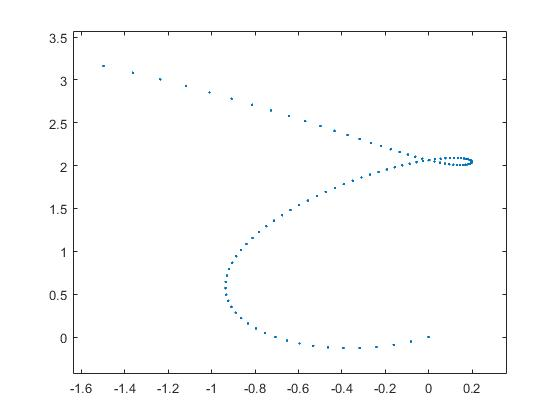
\includegraphics[width=\linewidth]{konstDt.jpg}
			\caption{$\Delta t=konst.$}
			\label{fig:constDt}
		\end{subfigure}%
	
		\begin{subfigure}{.5\textwidth}
			\centering
			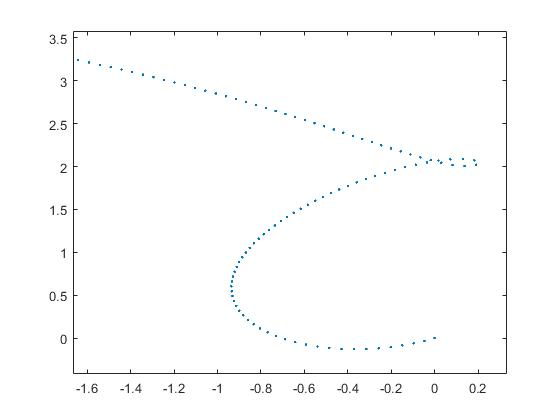
\includegraphics[width=\linewidth]{konstDs.jpg}
			\caption{$\Delta s=konst.$}
			\label{fig:constDs}
		\end{subfigure}
		\caption{Enakomerno povečanje parametra krivulje s PH (levo) in dolžine loka (desno) - parametrizacija po nekaj iteracijah. Prikaz točk na krivulji.}
		\label{fig:constD}
	\end{figure}
	
	\section{Lastnosti odvoda krivulje}
	Ker je parametrična hitrost krivulje s PH $r (t)$ definirane z integracijo polinom v $t$, imajo osnovne lastnosti njenih odvodov - enotski tangentni vektor, normala in ukrivljenost - racionalno odvisnost od parametra krivulje. Natančneje, definirani so v smislu polinomov $u (t)$ in $v (t)$, kjer
	$$\textbf{t} =\frac{(u^2 - v^2, 2uv)}{\sigma},\hspace{10pt} \textbf{n} =\frac{(2uv, v^2 - u^2)}{\sigma},\hspace{10pt} \kappa = 2 \frac{uv\prime - u\prime v}{\sigma^2}.$$
	
	\section{Racionalni odmiki krivulj s PH}
	Odmiki pri vsaki razdalji $d$ od krivulje s PH $r (t)$, definirani kot
	$$r_d (t) = r (t) + d \textbf{n} (t),$$
	dovoljujejo natančno predstavitev v smislu racionalnih B\'ezierjevevih krivulj, ker je enotska normala $\textbf{n} (t)$ racionalno odvisna od parametra krivulje $t$. 
	
	Naj bodo kontrolne točke krivulje s PH $r (t)$ zapisane v homogenih koordinatah kot
	$$\textbf{P}_k = (W_k, X_k, Y_k) = (1, x_k, y_k),\hspace{20pt} k = 0,\ldots , n.$$
	Definirajmo prve diference kot
	$$\Delta\textbf{P}_k = \textbf{P}_{k + 1} - \textbf{P}_k = (0, \Delta x_k, \Delta y_k),\hspace{20pt} k = 0,\ldots, n - 1$$
	kjer je $\Delta x_k = x_{k + 1}- x_k, \Delta y_k = y_{k + 1}- y_k$. Naj bo $\Delta\textbf{P}_k^\perp = (0, \Delta y_k, -\Delta x_k).$
	
	Odmik za razdaljo $d$ od krivulje s PH $r (t)$ je definiran zgoraj z $r_d(t)$, kjer je normala $\textbf{n}(t)$ na $r (t)$ podana zgoraj. Odmik lahko izrazimo kot
	$$r_d (t) = \left(\frac{X (t)}{W(t)},\frac{Y(t)}{W(t)}\right),$$
	kjer so $W (t), X (t), Y (t)$ polinomi stopnje $2n - 1$, katerih koeficienti
	$$\textbf{O}_k = (W_k, X_k, Y_k), \hspace{10px} k = 0,\ldots , 2n - 1,$$
	določajo B\'ezierjeve kontrolne točke racionalne krivulje odmika.
	
	Homogene koordinate za kontrolne točke odmika so lahko strnjeno izražene v smislu prvotne krivulje kot
	$$\textbf{O}_k =\sum^{min (n - 1, k)}_{j = max (0, k - n)}\frac{\binom{n-1}{j}\binom{n}{k-j}}{\binom{2n-1}{k}}(\sigma_j\textbf{P}_{k-j}+dn\Delta\textbf{P}_j^\perp),$$ $$k = 0,\ldots, 2n - 1.$$
	
	S tem dobimo za kubične krivulje s PH 6 kontrolnih točk racionalnih odmikov kot krivulj pete stopnje, za krivulje s PH pete stopnje pa dobimo 10 kontrolnih točk racionalnih odmikov kot krivulj devete stopnje.
	
	\centering
	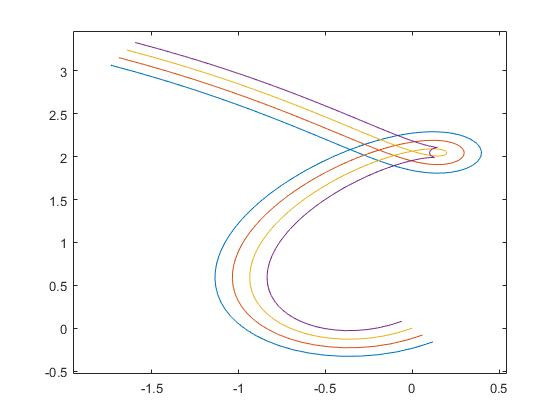
\includegraphics[width=\linewidth]{odmik.jpg} \captionof{figure}{Krivulja s PH (rumena) in racionalni odmiki za $d=-0.2,-0.1,0.1$.}
	\label{fig:odmik}
	
	Opazimo, da so racionalni odmiki eksaktni za vsak $d$ tudi v primeru špic in ko krivulja prečka samo sebe.
	
	\section{Nadaljevanje}
	Obravnava 19. poglavja, implementacija 19 poglavja v Matlab in zaključek
	
	\begin{thebibliography}{1}
		\bibitem{knjiga} R. T. Farouki: Pythagorean-Hodograph Curves: Algebra and Geometry Inseparable, poglavje 17 in 19.
	\end{thebibliography}
\end{document}